\chapter{實驗設定與結果}
\label{c:experiment}

在這一章中,我們會先介紹我們在實驗中所使用到的資料集,然後說明我們在訓練和測試時使用的設定與參數,接著展示我們進行測試所獲得在數據與視覺上的結果,最後展示對我們的方法進行消熔實驗的結果與討論。

\section{資料集}

我們在實驗中所使用到的資料集主要分為訓練用和測試用的資料集。

\begin{figure}[t]
\centering
\begin{subfigure}[b]{0.3\textwidth}
    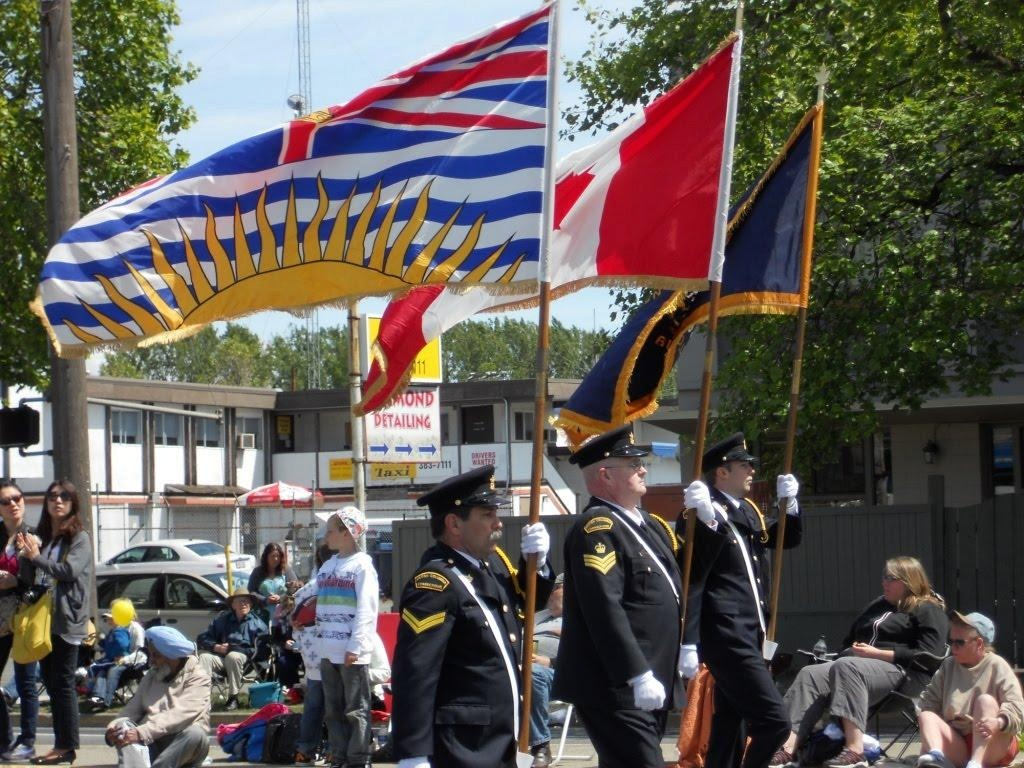
\includegraphics[width=\textwidth]{figures/wider_1}
\end{subfigure}
\begin{subfigure}[b]{0.3\textwidth}
    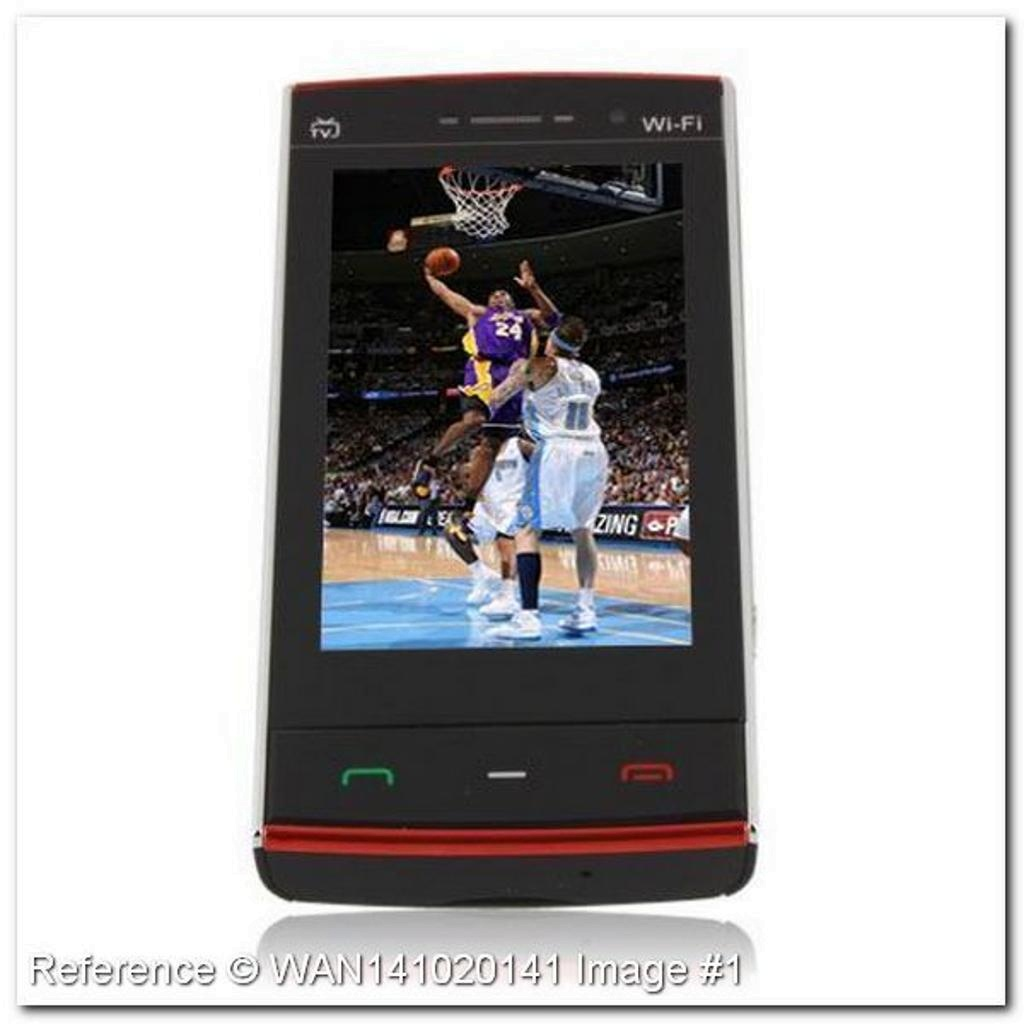
\includegraphics[width=\textwidth]{figures/wider_2}
\end{subfigure}
\begin{subfigure}[b]{0.3\textwidth}
    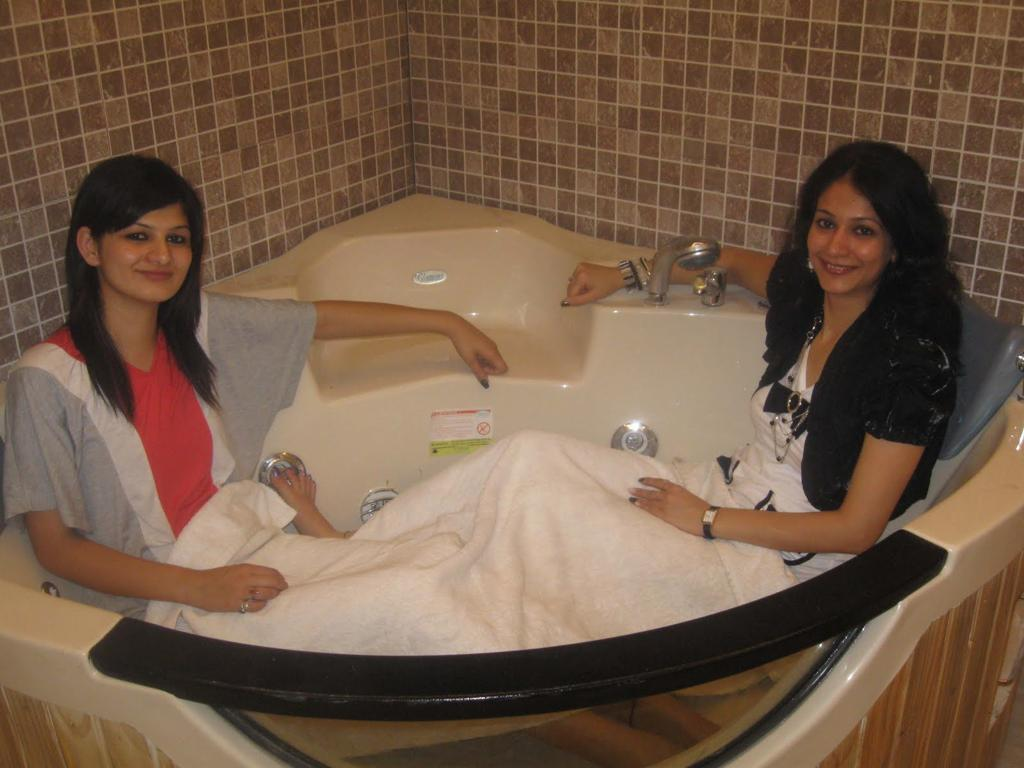
\includegraphics[width=\textwidth]{figures/wider_3}
\end{subfigure}
\begin{subfigure}[b]{0.3\textwidth}
    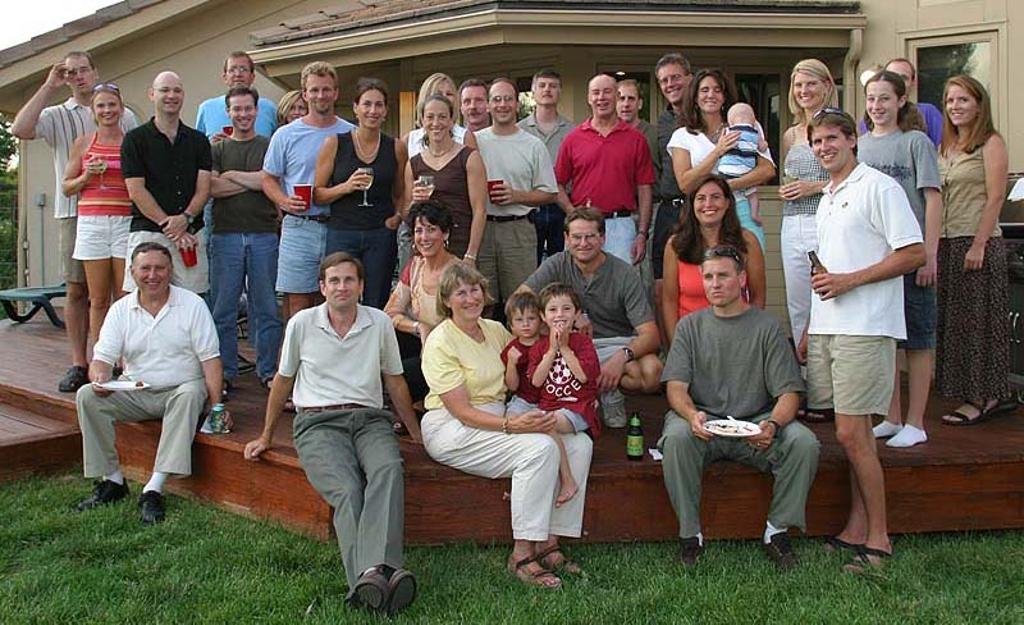
\includegraphics[width=\textwidth]{figures/wider_4}
\end{subfigure}
\begin{subfigure}[b]{0.3\textwidth}
    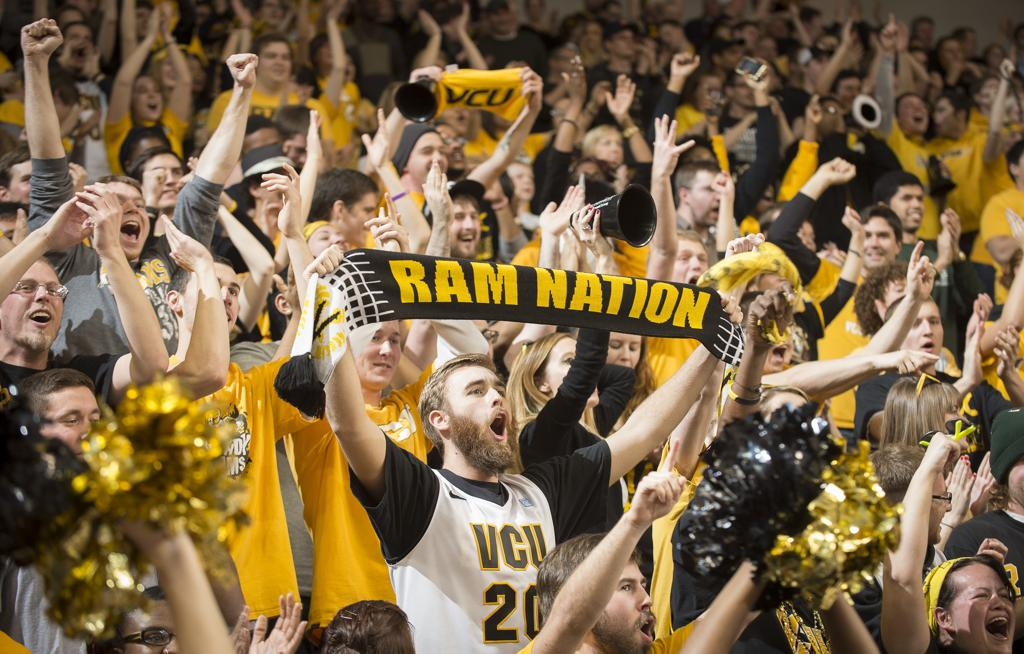
\includegraphics[width=\textwidth]{figures/same_original}
\end{subfigure}
\caption[Wider Face 資料集中的圖片範例]{Wider Face 資料集收集了各種不同情境下的人臉}
\label{fig:wider_face}
\end{figure}

訓練時我們使用了 Wider Face~\cite{yang2016wider} 作為主要的資料集。它是一個人臉資料集,其收集了各種不同情境下的人臉 (如圖~\ref{fig:wider_face}),共計 32,203 張圖片、393,703 張人臉,在人臉偵測這個議題上是很經典的資料集。在我們的實驗中,我們將資料集中的圖片分別做了曝光不足和曝光過度的模擬。其中曝光不足的模擬將圖片亮度隨機調為3\%、5\%、7\%,並將每張圖隨機分配 1 \textasciitilde 10 的數字$n$,以$\sigma = n$的設定對每張圖做高斯雜訊;曝光過度的模擬則將圖片亮度隨機調為100\%、250\%、400\%。

\begin{figure}[t]
\centering
\begin{subfigure}[b]{0.22\textwidth}
    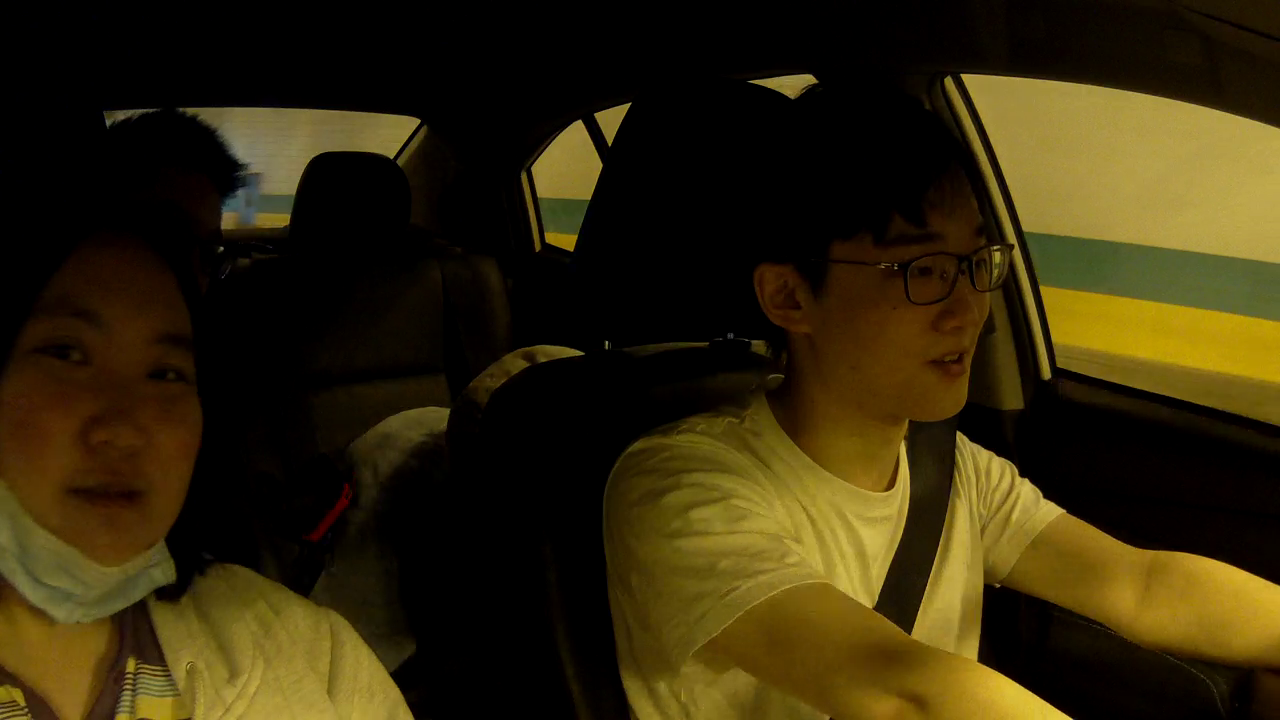
\includegraphics[width=\textwidth]{figures/test_1_1}
\end{subfigure}
\begin{subfigure}[b]{0.22\textwidth}
    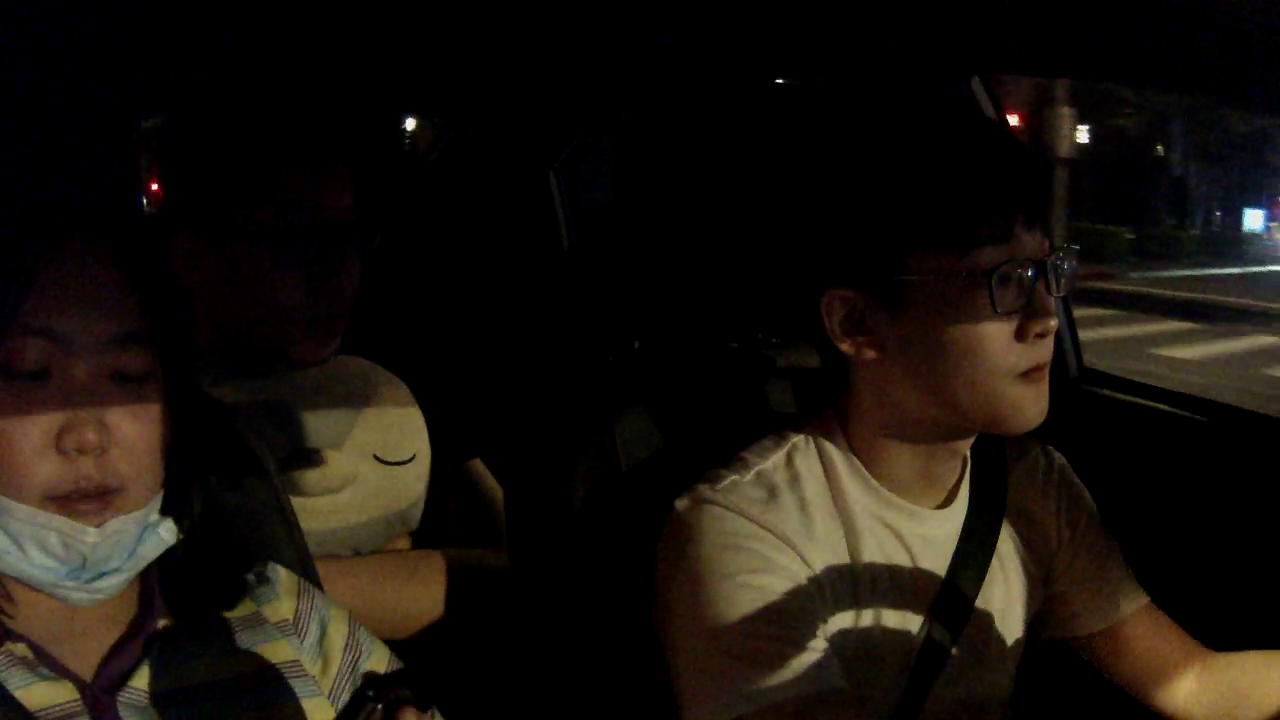
\includegraphics[width=\textwidth]{figures/test_2_1}
\end{subfigure}
\begin{subfigure}[b]{0.22\textwidth}
    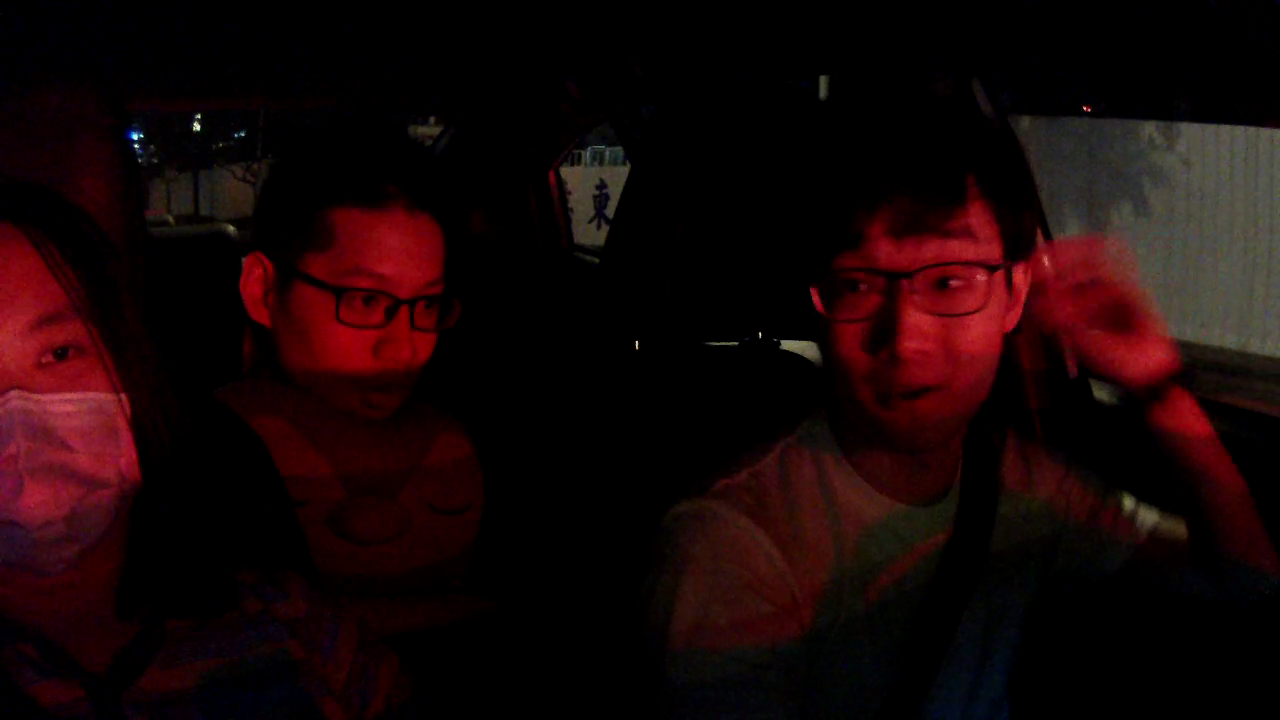
\includegraphics[width=\textwidth]{figures/test_3_1}
\end{subfigure}
\begin{subfigure}[b]{0.22\textwidth}
    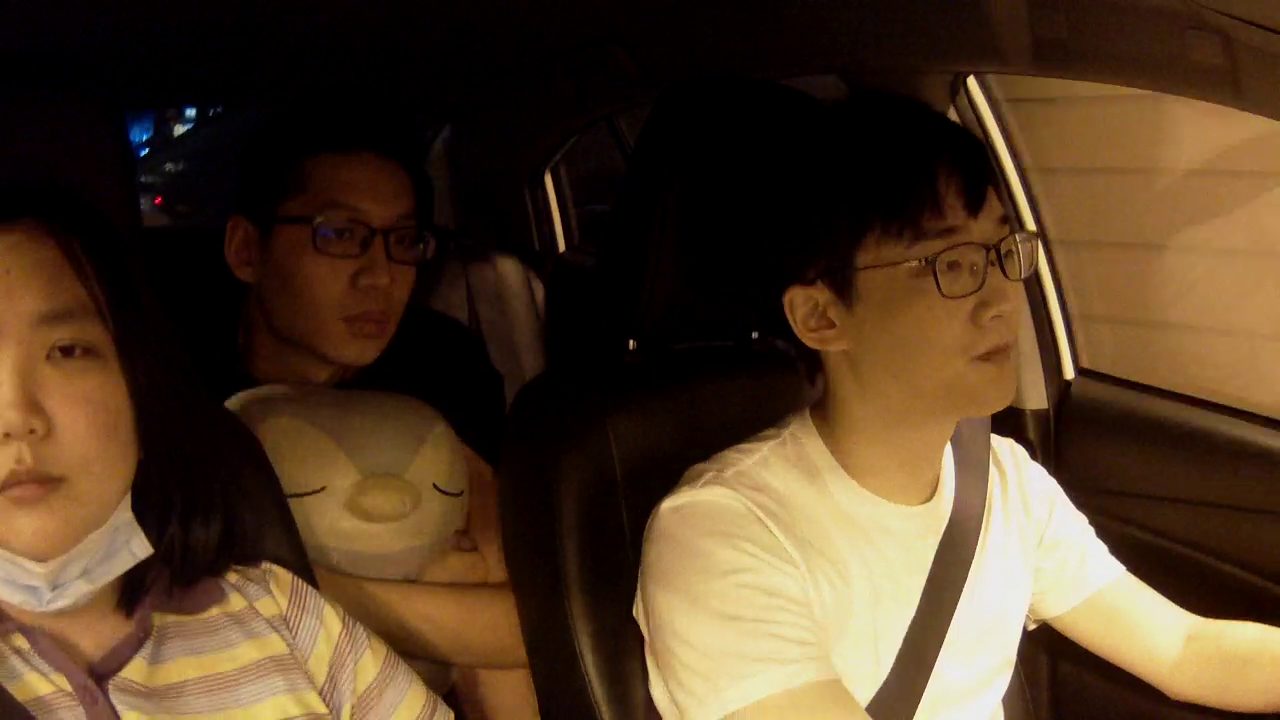
\includegraphics[width=\textwidth]{figures/test_4_1}
\end{subfigure}
\begin{subfigure}[b]{0.22\textwidth}
    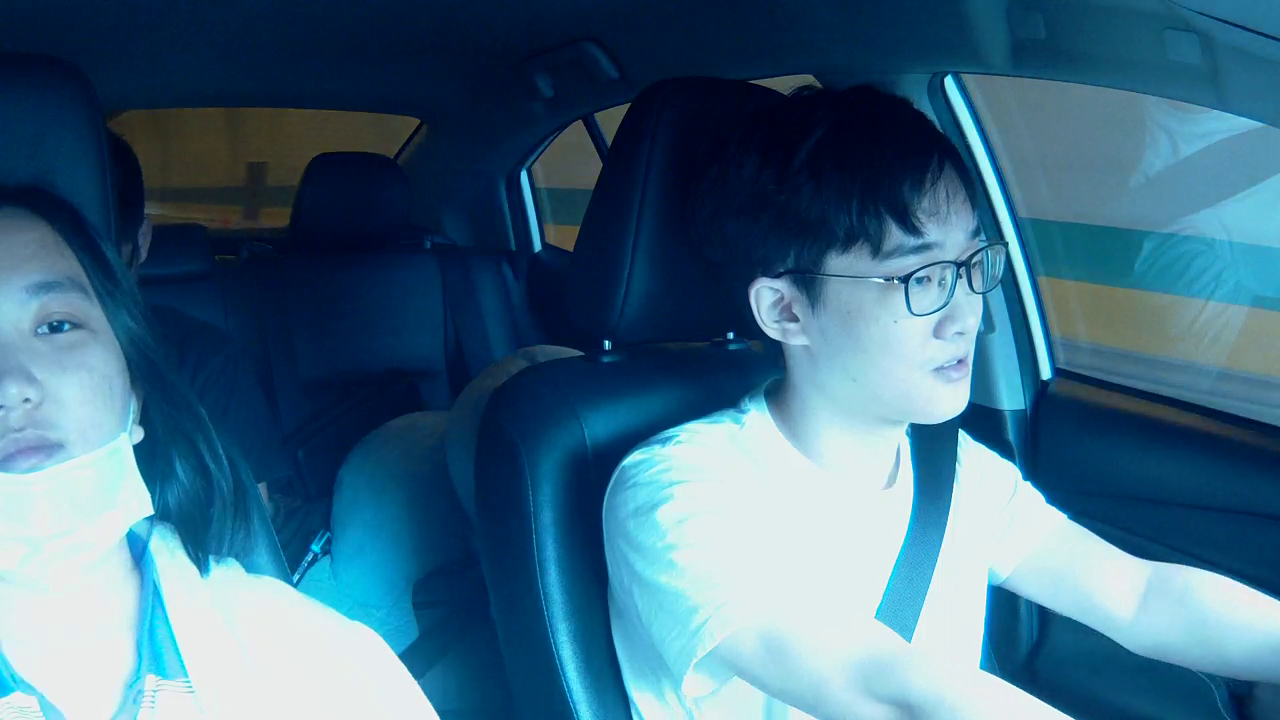
\includegraphics[width=\textwidth]{figures/test_1_2}
    \caption {白天進出隧道}
\end{subfigure}
\begin{subfigure}[b]{0.22\textwidth}
    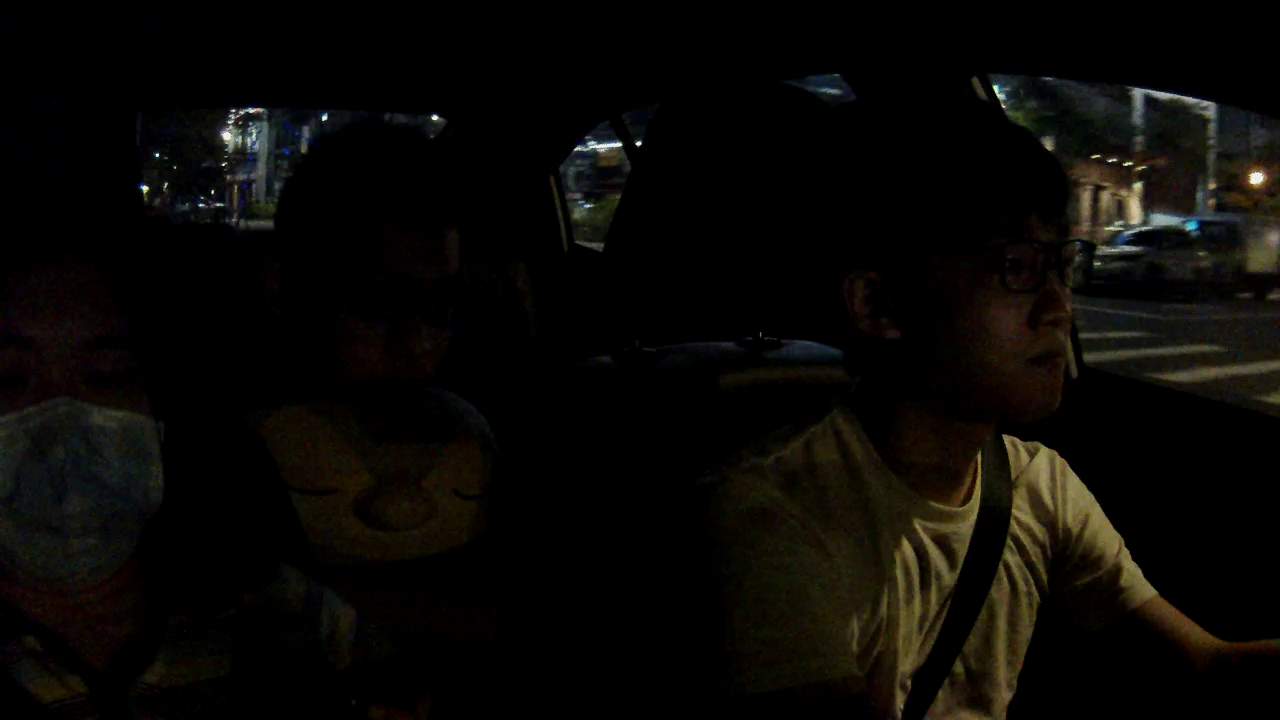
\includegraphics[width=\textwidth]{figures/test_2_2}
    \caption {夜間極暗}
\end{subfigure}
\begin{subfigure}[b]{0.22\textwidth}
    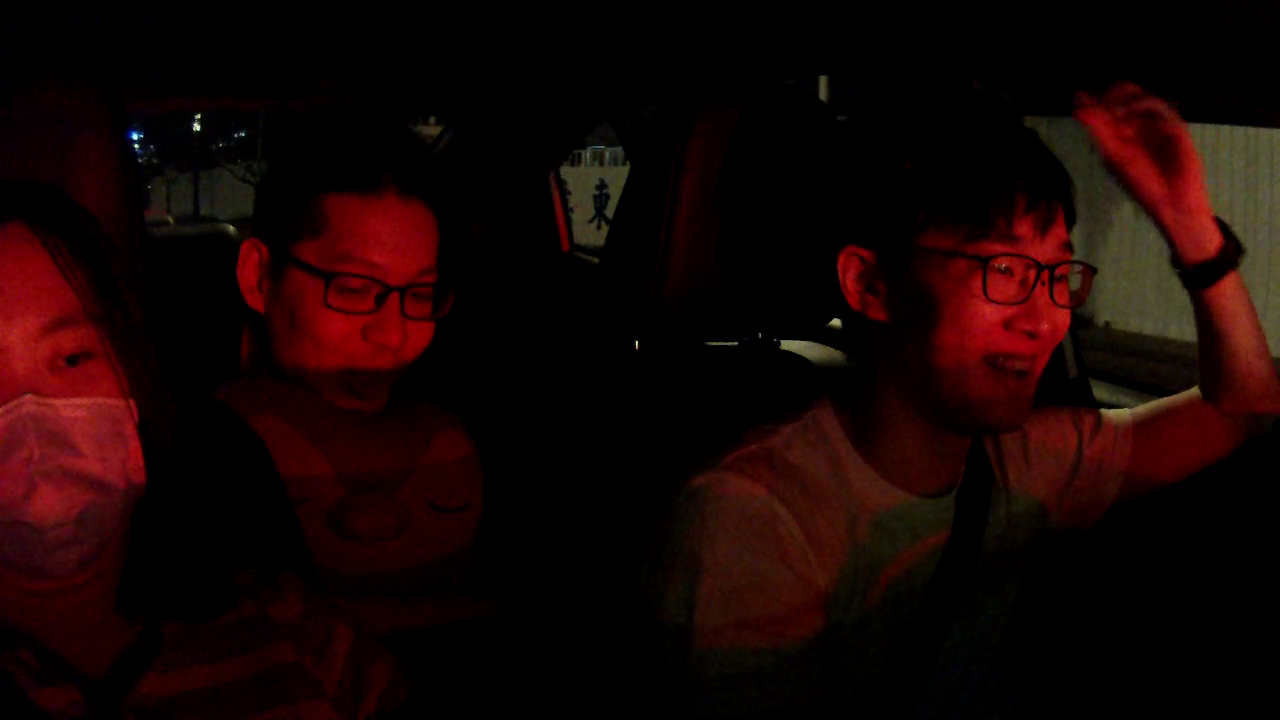
\includegraphics[width=\textwidth]{figures/test_3_2}
    \caption {夜間等紅燈}
\end{subfigure}
\begin{subfigure}[b]{0.22\textwidth}
    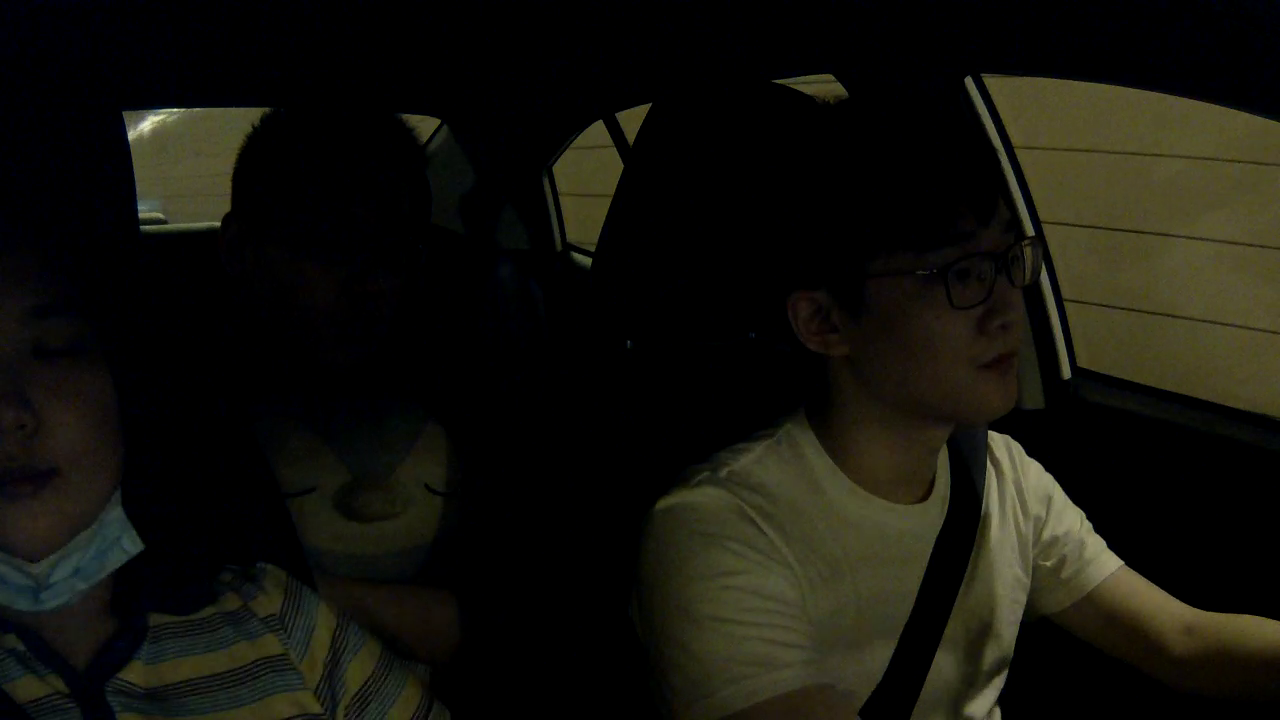
\includegraphics[width=\textwidth]{figures/test_4_2}
    \caption {夜間隧道內}
\end{subfigure}
\caption[測試資料集中的圖片範例]{測試資料集中包含白天進出隧道、夜間極暗、夜間等紅燈和夜間隧道內四個情境}
\label{fig:test_data}
\end{figure}

測試時我們則使用了自己拍攝的車內影像。我們在進行拍攝時將 Patriot F5 置於前擋風玻璃右上角,影像解析度為$1280 \times 720$,幀率為 30 fps。影像中會出現三個人,包含駕駛、副駕駛、後座的乘客。此資料集有以下四個情境:白天進出隧道 900 張、夜間極暗 900 張、夜間等紅燈 900 張、夜間隧道內 1000 張 (如圖~\ref{fig:test_data})。白天進出隧道是四個情境中最亮的,用來測試進出隧道時的光線劇烈變化造成的影響;夜間極暗是一個環境光非常微弱的情境,用來測試缺乏環境光造成的影響;夜間等紅燈是一個會受到紅燈直接照射的情境,用來測試資料有色差造成的影響;夜間隧道內是一個隧道光源較微弱的情境,用來測試環境光僅能照亮部分影像造成的影響。在後續的實驗我們也會將這四個情境分開測試。
為求說明方便,後續提到資料集時會使用表~\ref{table:model_names}中對資料集的命名。
\begin{table}[ht]
    \caption{對不同資料集的命名}
    \centering
    \begin{tabular}{l l l}
        \hline
        資料集名稱 & 說明 & 使用時機 \\
        \hline
        $D_{Original}$ & Wider Face 的原始資料集 & - \\
        $D_{Dark}$ & 將 $D_{Original}$ 做曝光不足模擬後的資料集 & - \\
        $D_{Bright}$ & 將 $D_{Original}$ 做曝光過度模擬後的資料集 & - \\
        $D_{Triple}$ & 包含 $D_{Original}$、$D_{Dark}$、$D_{Bright}$ 三個資料集 & 預訓練 \\
        $D_{Train}$	& 包含 $D_{Dark}$ 和 $D_{Bright}$ 兩個資料集 & 主要訓練 \\
        $D_{Test}$ & 我們拍攝的車內影像 & 測試 \\
        \hline
    \end{tabular}
    \label{table:model_names}
\end{table}

\section{實驗設定}

訓練的流程包含預訓練和主要訓練。

在預訓練中,我們使用 $D_{Triple}$ 作為輸入資料集。首先我們將每張圖片調整為 $1024 \times 1024$ 的大小以配合後續訓練要求,然後將圖片切為 256 張 $64 \times 64$ 的小圖片餵進模型以 $\alpha = 0.05$ 進行訓練,經過30萬個時期 (Epoch) 後得到正規器在主要訓練中的初始權重。
接著我們進行主要訓練,在這個階段我們使用$D_{Train}$作為輸入資料集,把預訓練中得到的正規器和人臉偵測器接在一起做150個時期的端對端訓練。
測試時我們使用 $D_{Test}$ 作為輸入資料集,對其四個情境分別進行測試和結果評估。

\section{實驗結果}

以下會展示用我們的方法測試的結果和用基線測試的結果在數據和視覺上的比較。基線是用將 FaceBoxes 的架構以和原論文中同樣的資料集 ($D_{Original}$) 訓練得到的模型直接對 $D_{Test}$ 進行測試,並已事先測試過該模型做在論文中提到的測試資料上結果和原論文結果相似。
數據上的結果比較如表~\ref{table:baseline_compare},表中數據是我們使用召回率 (Mean Average Precision) 對偵測結果計算得出的數字,並已經去除部分和本研究無關的結果影響。
\begin{table}[ht]
    \caption{基線和我們的方法之結果比較}
    \centering
    \begin{tabular}{l c c c c}
        \hline
        模型名稱 & 白天進出隧道 & 夜間極暗 & 夜間等紅燈 & 夜間隧道內 \\
        \hline
        基線 & 63.54\% & 31.70\% & 93.35\% & 47.46\% \\
        我們的方法 & 76.25\% & 78.97\% & 97.51\% & 71.66\% \\
        \hline
    \end{tabular}
    \label{table:baseline_compare}
\end{table}

由數據結果可以發現我們的方法得出的結果在環境光較微弱的夜間極暗、夜間隧道內兩個情境下和基線相比有了顯著的進步,而在其他兩個情境則有小幅進步。從視覺上的結果 (如圖~\ref{fig:comp_with_base}) 也可看出我們的方法和基線相比能夠偵測出更多曝光不足的人臉,同時兼顧偵測受到正常光線照射下人臉的準確率。

\begin{figure}[t]
\centering
\begin{subfigure}[b]{0.45\textwidth}
    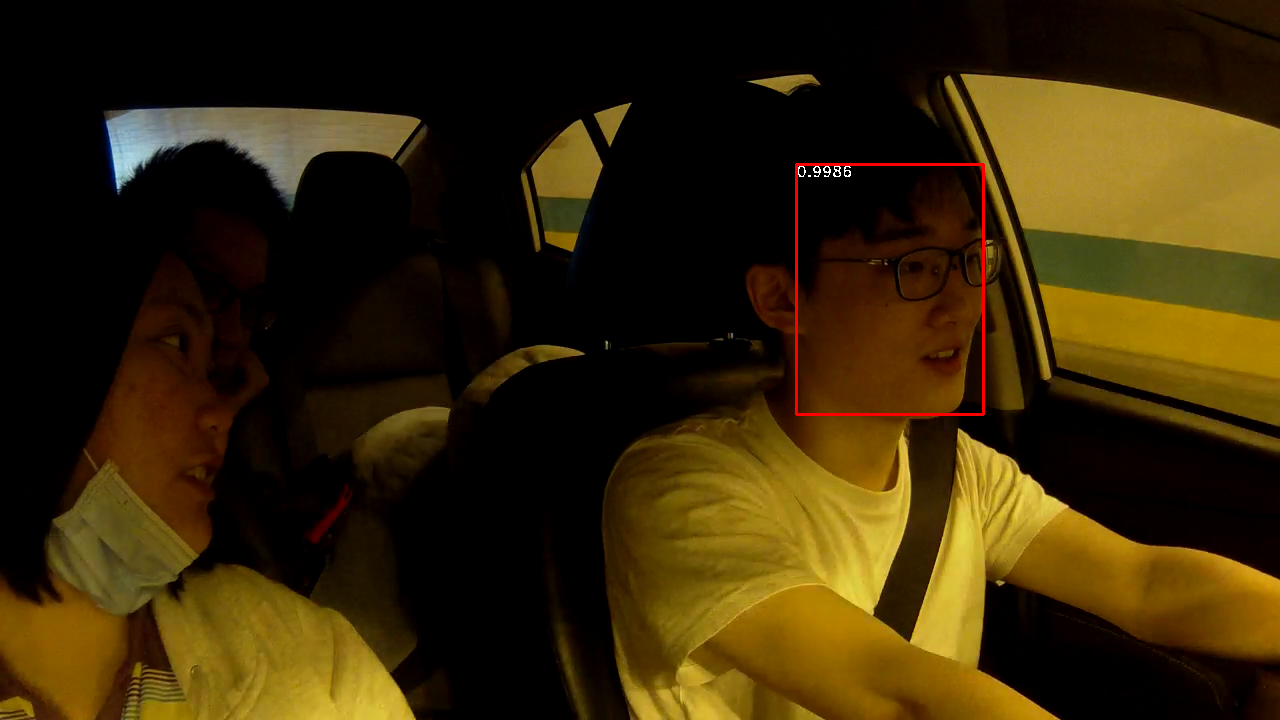
\includegraphics[width=\textwidth]{figures/comp_base1}
\end{subfigure}
\begin{subfigure}[b]{0.45\textwidth}
    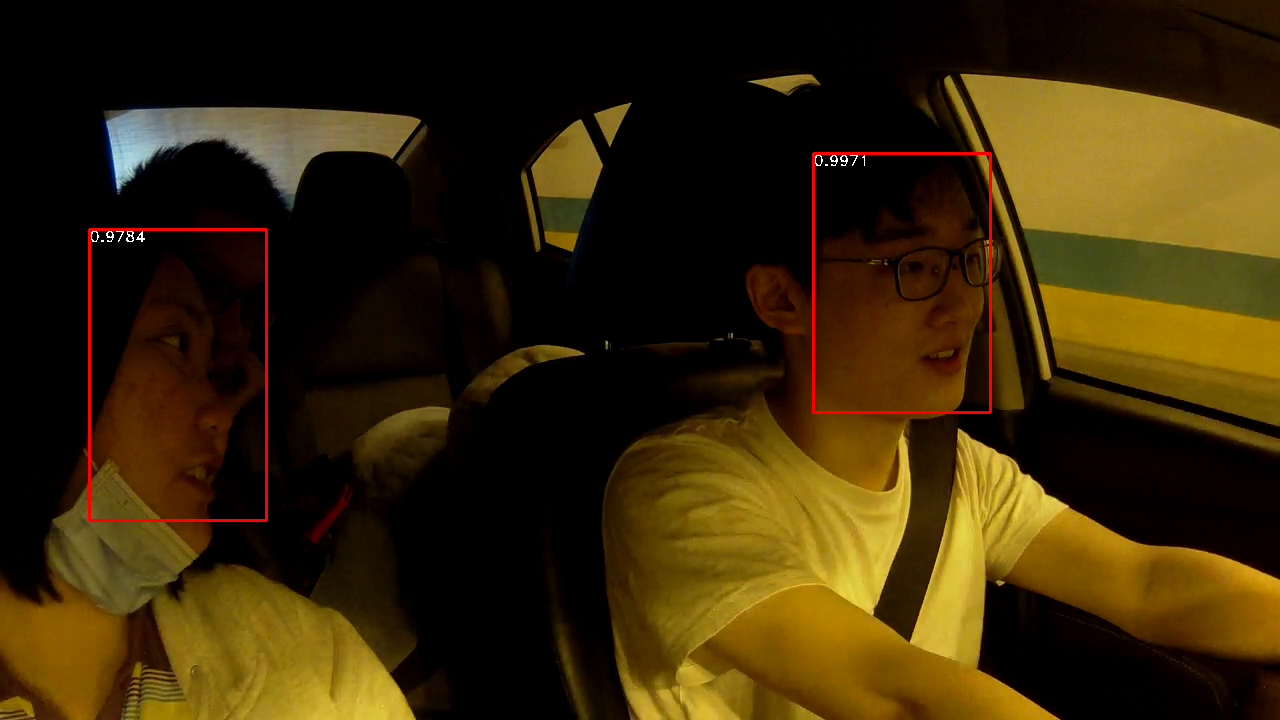
\includegraphics[width=\textwidth]{figures/comp_ours1}
\end{subfigure}
\begin{subfigure}[b]{0.45\textwidth}
    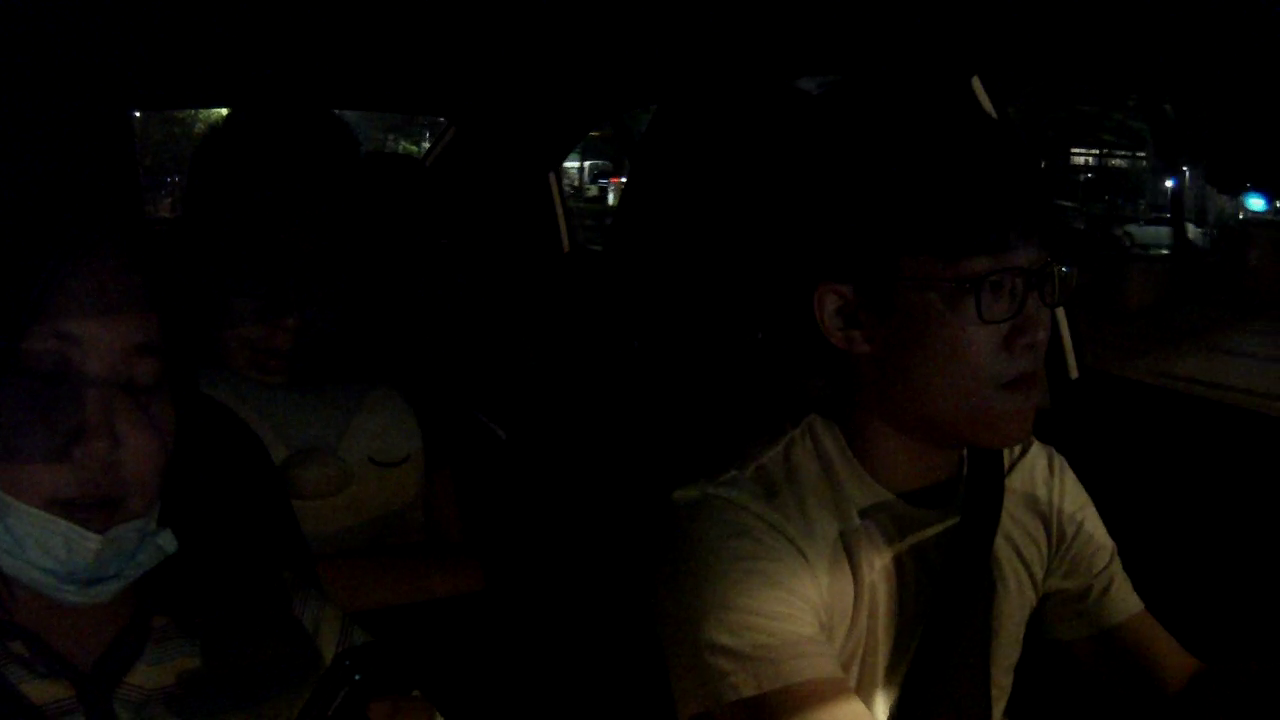
\includegraphics[width=\textwidth]{figures/comp_base2}
\end{subfigure}
\begin{subfigure}[b]{0.45\textwidth}
    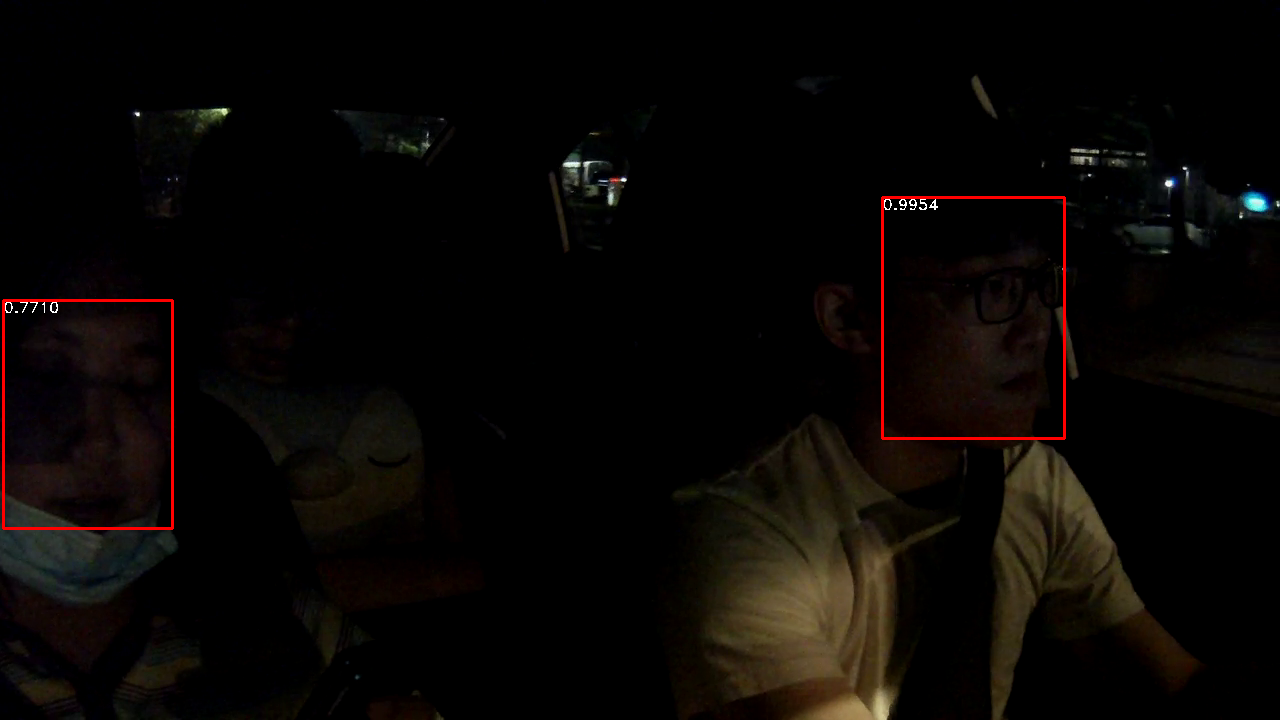
\includegraphics[width=\textwidth]{figures/comp_ours2}
\end{subfigure}
\begin{subfigure}[b]{0.45\textwidth}
    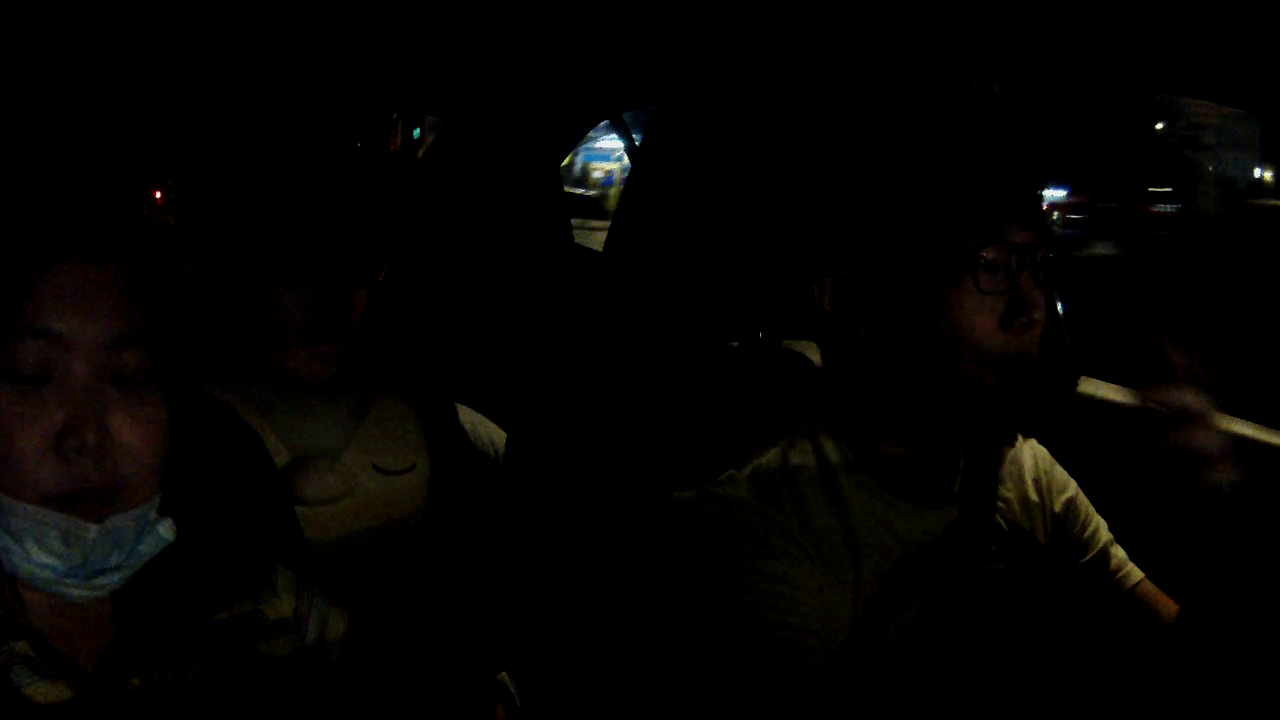
\includegraphics[width=\textwidth]{figures/comp_base3}
\end{subfigure}
\begin{subfigure}[b]{0.45\textwidth}
    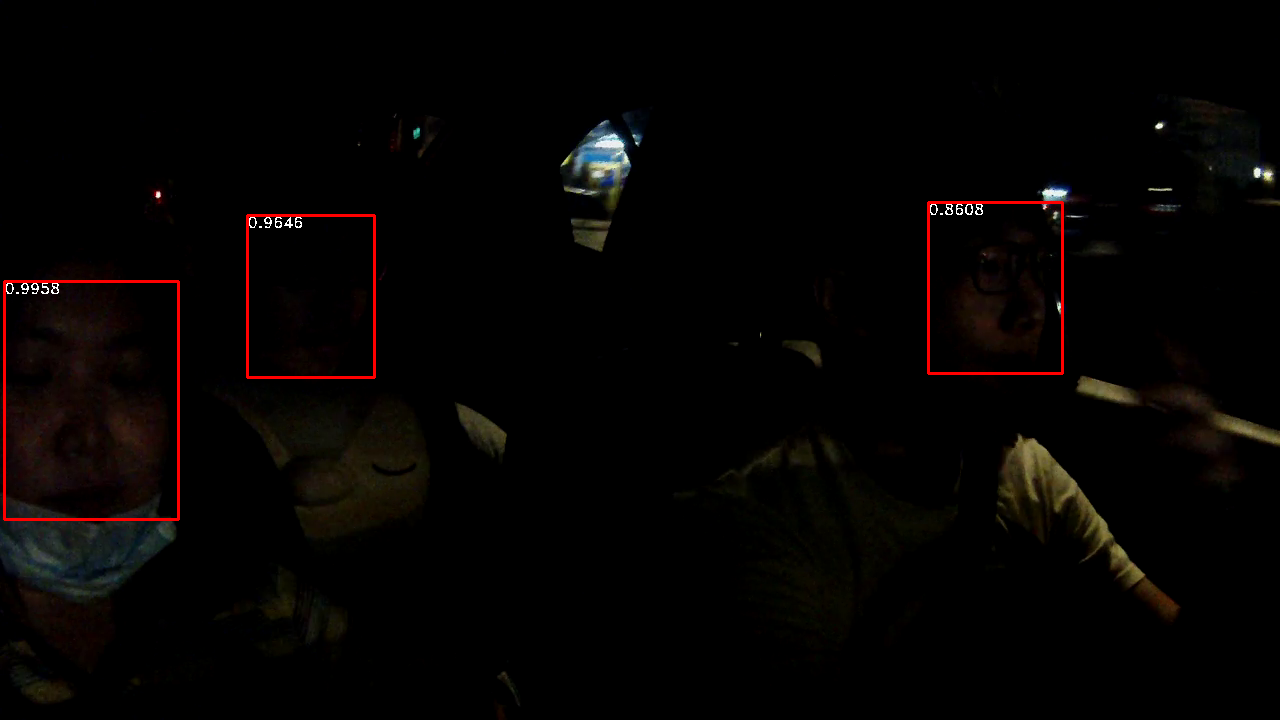
\includegraphics[width=\textwidth]{figures/comp_ours3}
\end{subfigure}
\begin{subfigure}[b]{0.45\textwidth}
    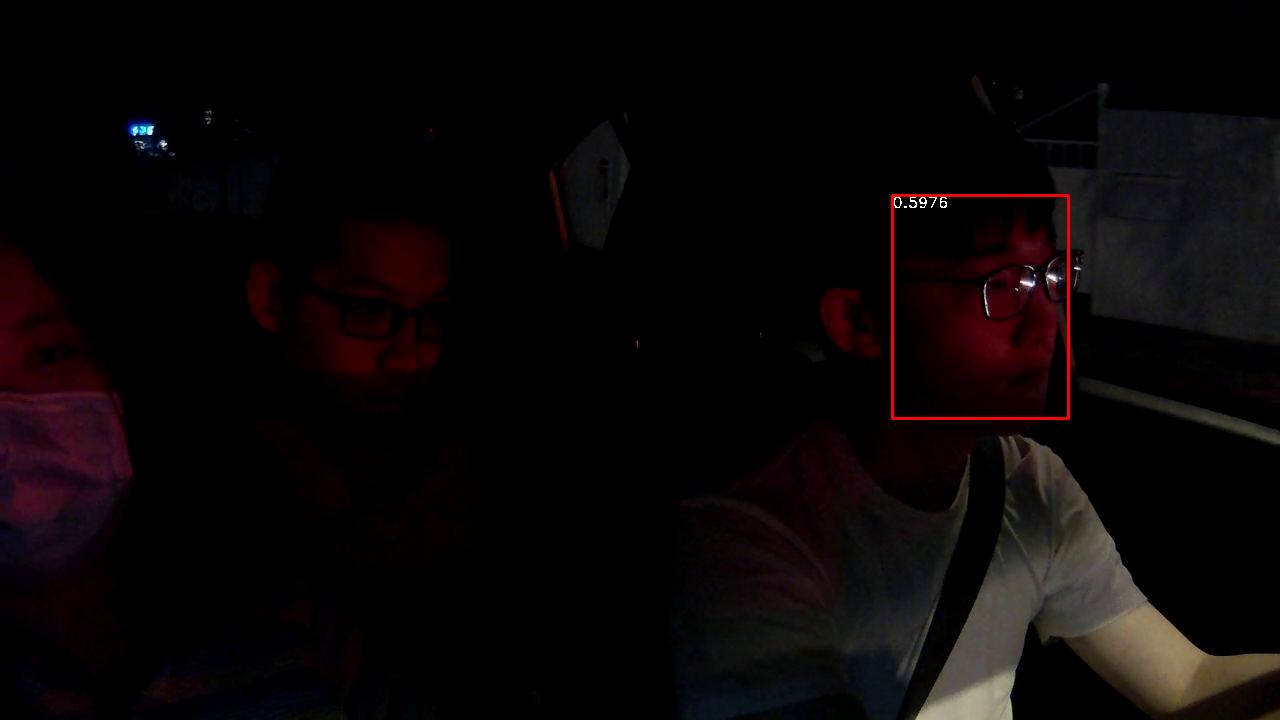
\includegraphics[width=\textwidth]{figures/comp_base4}
\end{subfigure}
\begin{subfigure}[b]{0.45\textwidth}
    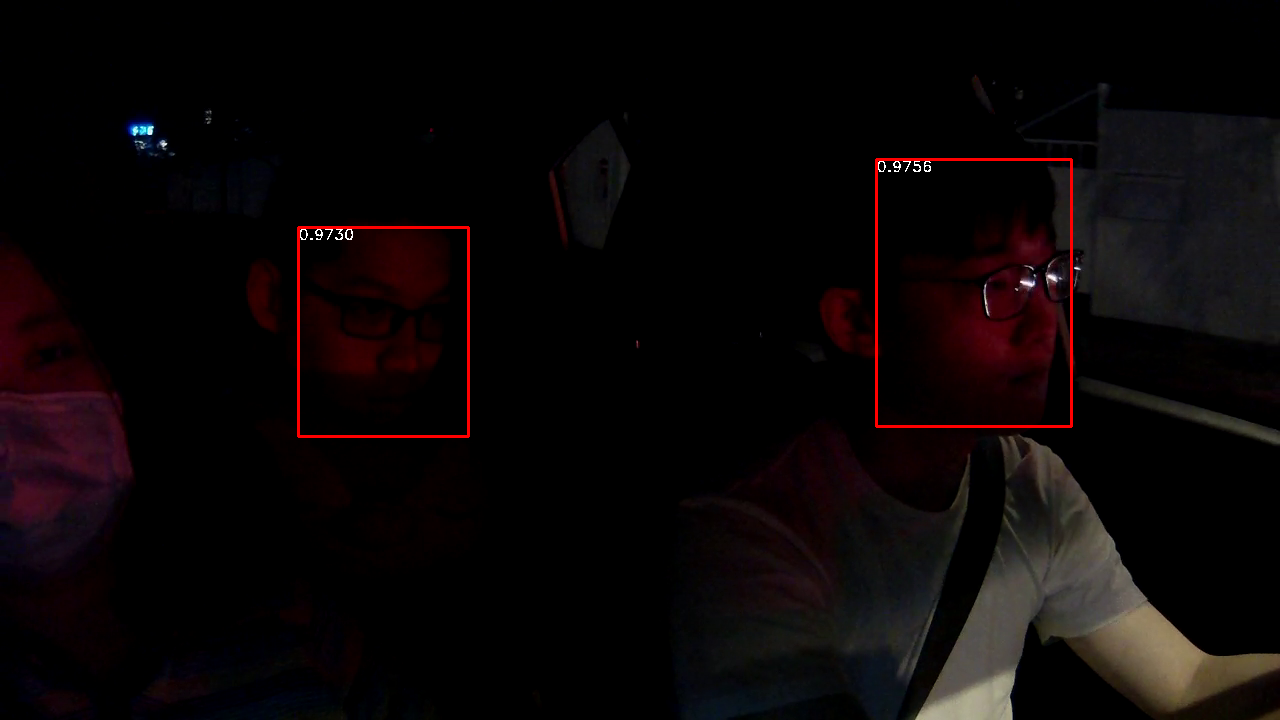
\includegraphics[width=\textwidth]{figures/comp_ours4}
\end{subfigure}
\begin{subfigure}[b]{0.45\textwidth}
    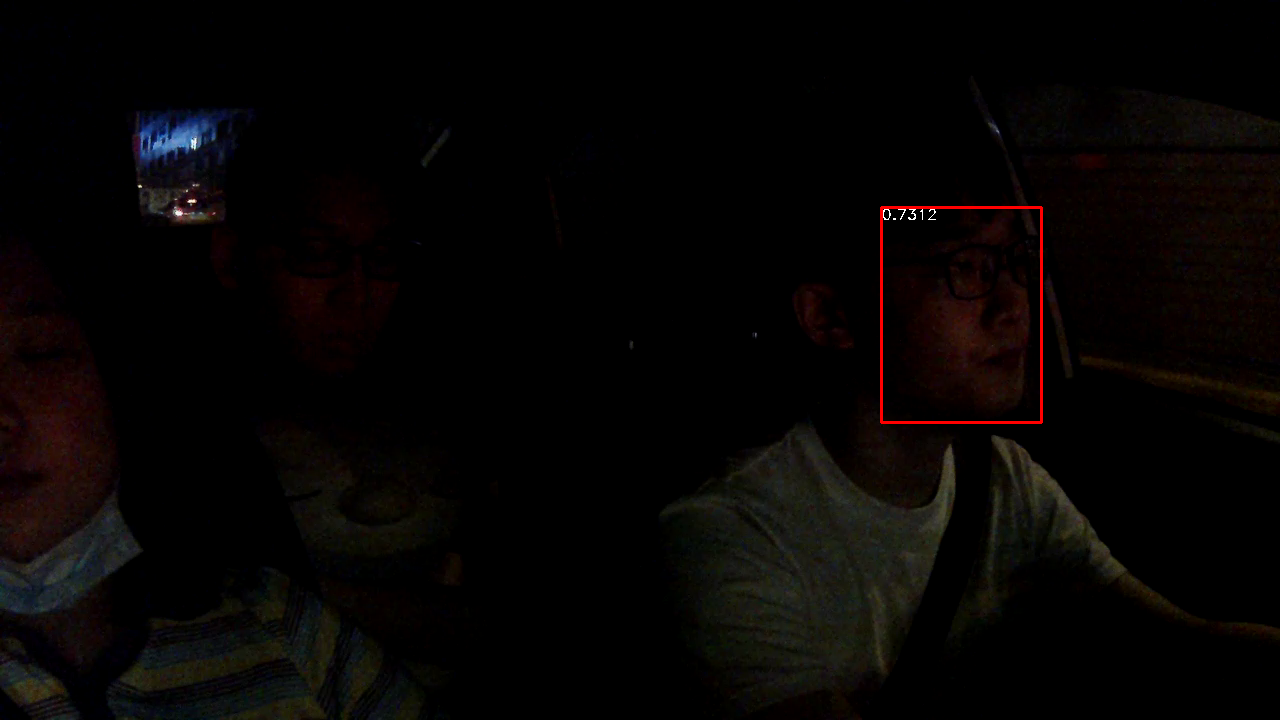
\includegraphics[width=\textwidth]{figures/comp_base5}
\end{subfigure}
\begin{subfigure}[b]{0.45\textwidth}
    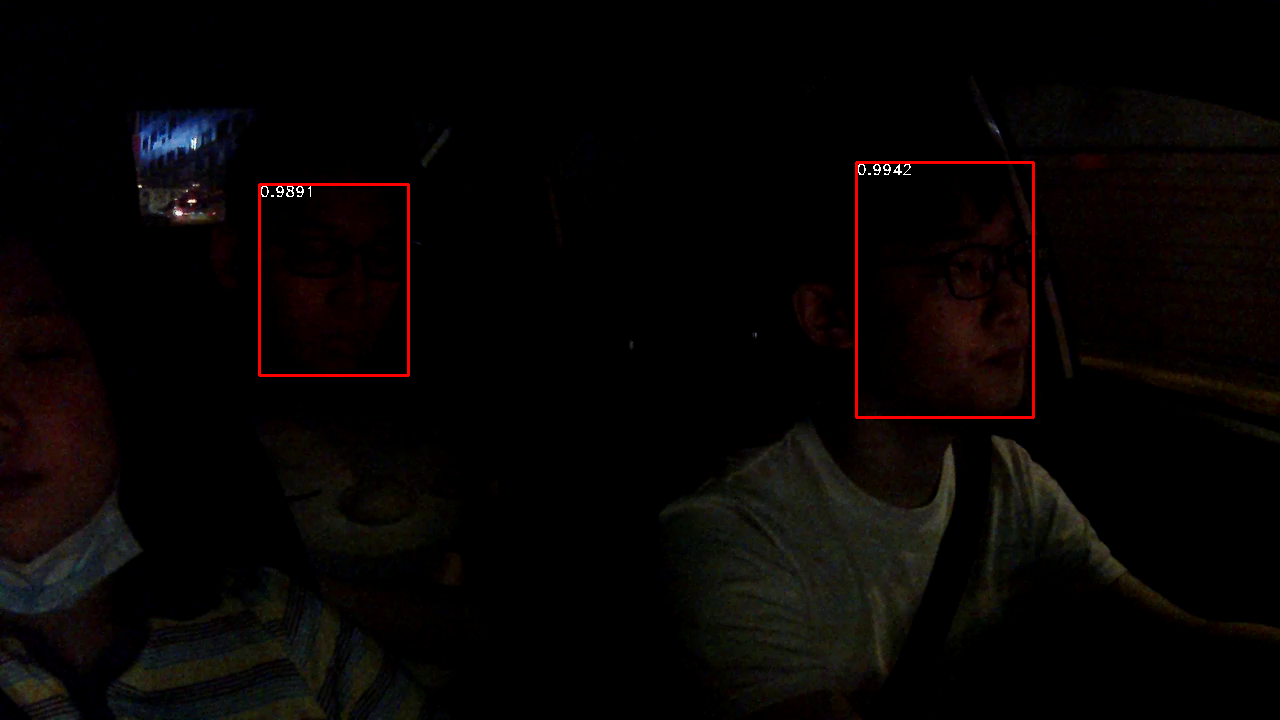
\includegraphics[width=\textwidth]{figures/comp_ours5}
\end{subfigure}
\begin{subfigure}[b]{0.45\textwidth}
    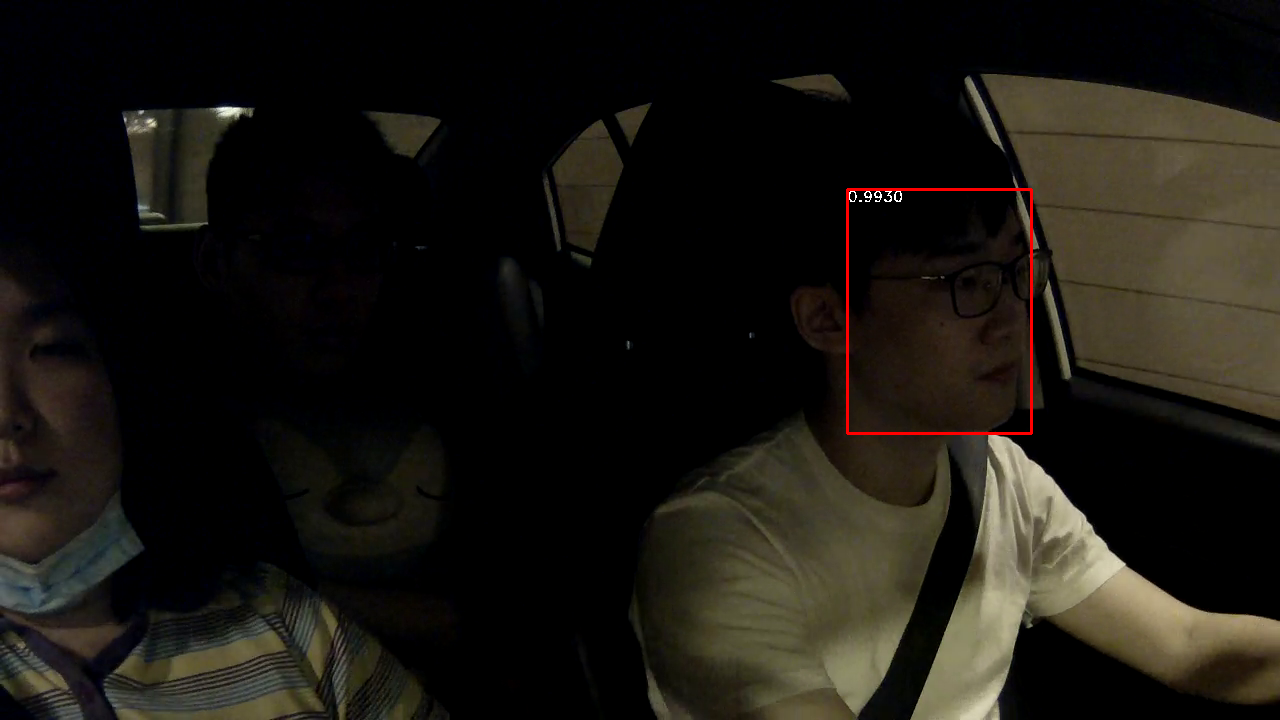
\includegraphics[width=\textwidth]{figures/comp_base6}
    \caption {基線的測試結果}
\end{subfigure}
\begin{subfigure}[b]{0.45\textwidth}
    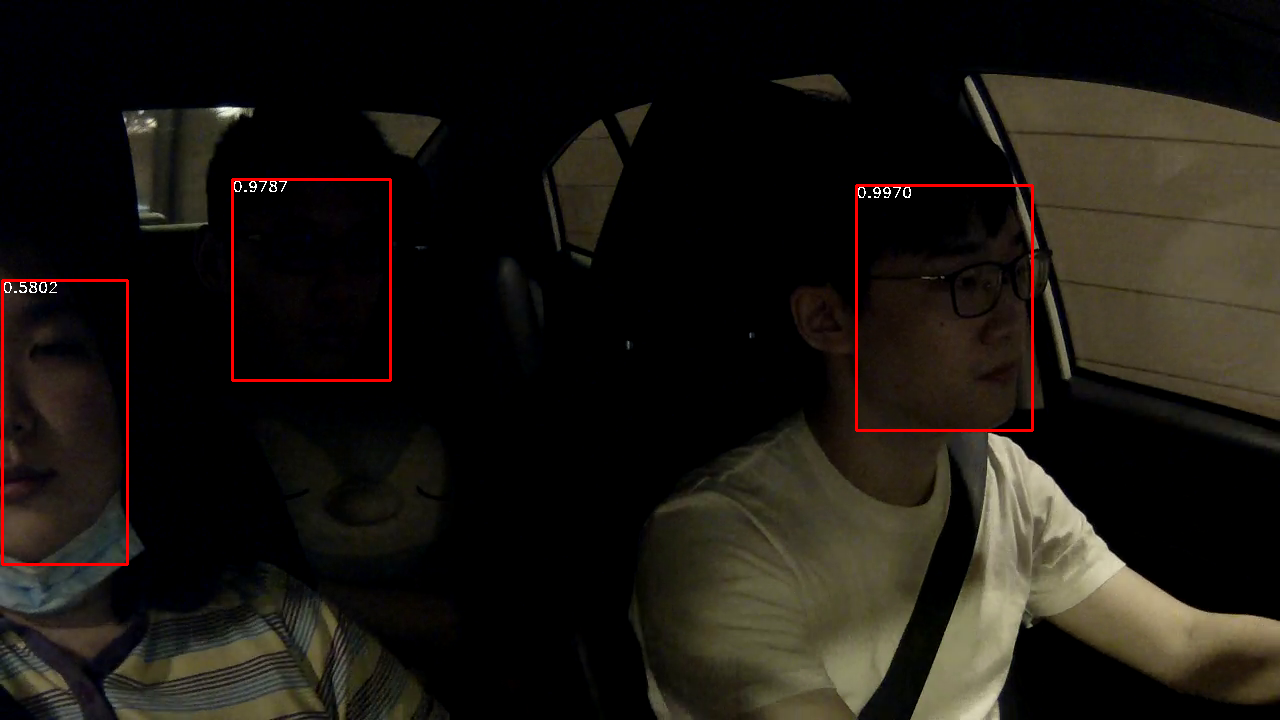
\includegraphics[width=\textwidth]{figures/comp_ours6}
    \caption {我們的方法的測試結果}
\end{subfigure}
\caption[我們的方法與基線之視覺結果比較]{比較我們的方法與基線之視覺結果可發現我們的方法能偵測出更多曝光不足的人臉}
\label{fig:comp_with_base}
\end{figure}

\section{消融實驗}

在這一節我們會進行各種不同訓練設定下的測試,來確認我們的方法的各個步驟都是有效的。首先我們會先介紹在這一節中會用到的幾個訓練設定的細節,然後再展示數據間比較的結果並進行討論。

以下的設定包含了基線、雙倍資料、預訓練基線方法、預訓練基線端對端優化、原圖預訓練端對端優化、三圖預訓練、我們的方法這七個設定。基線方法和我們的方法在前面已經提過;雙倍資料是建立在基線上,將訓練的資料集從 $D_{Original}$ 換成 $D_{Train}$ 的設定;預訓練基線方法是我們用 python 實作了 MSR-net 這篇論文的方法後,以經過視網膜增強算法處理 $D_{Dark}$ 後的圖片作為參考圖用 $D_{Dark}$ 訓練出正規器,固定正規器的權重後和人臉偵測器接在一起用$D_{Train}$訓練偵測器權重的設定;預訓練基線端對端優化則是預訓練和前個設定相同,但在主要訓練的階段進行端對端優化的設定;原圖預訓練端對端優化則在預訓練時以Doriginal作為Dtrain的參考圖訓練,主要訓練階段時以$D_{Train}$進行端對端訓練的設定;三圖預訓練是在預訓練階段用三圖一組架構訓練,但主要訓練階段固定正規器的權重僅訓練偵測器權重的設定。
\begin{table}[ht]
    \caption{不同設定間之結果比較}
    \centering
    \begin{tabular}{l c c c c}
        \hline
        模型名稱 & 白天進出隧道 & 夜間極暗 & 夜間等紅燈 & 夜間隧道內 \\
        \hline
        基線 & 63.54\% & 31.70\% & 93.35\% & 47.46\% \\
        雙倍資料 & 70.97\% & 63.16\% & 90.75\% & 62.73\% \\
        預訓練基線 & 73.15\% & 60.13\% & 88.67\% & 63.88\% \\
        預訓練基線端對端優化 & 74.66\% & \textbf{81.21\%} &95.42\% & 69.54\% \\
        原圖預訓練端對端優化 & 73.56\% & 76.02\% & 96.59\% & 68.73\% \\
        三圖預訓練 & 22.61\% & 41.13\% & 83.31\% & 30.35\% \\
        我們的方法 & \textbf{76.25\%} & 78.97\% & \textbf{97.51\%} & \textbf{71.66\%} \\
        \hline
    \end{tabular}
    \label{table:all_compare}
\end{table}
接下來我們分別對修改訓練資料集、在偵測前進行正規化處理、使用三圖一組架構進行預訓練、在預訓練後對正規器進行端對端訓練優化的成效進行比較與討論。

\subsection{修改訓練資料集}

我們比較基線和雙倍資料這兩個設定的結果如表~\ref{table:data_compare},這兩個設定只差在訓練時所使用的資料集,前者使用$D_{Original}$,後者使用 $D_{Train}$。

\begin{table}[ht]
    \caption{針對修改訓練資料集前後之比較}
    \centering
    \begin{tabular}{l c c c c}
        \hline
        模型名稱 & 白天進出隧道 & 夜間極暗 & 夜間等紅燈 & 夜間隧道內 \\
        \hline
        基線 & 63.54\% & 31.70\% & 93.35\% & 47.46\% \\
        雙倍資料 & 70.97\% & 63.16\% & 90.75\% & 62.73\% \\
        \hline
    \end{tabular}
    \label{table:data_compare}
\end{table}

我們發現使用較極端光線照射下的圖片作為輸入資料有助於讓偵測器認識更多在不同光線照射下的人臉,使能夠被偵測出的人臉數增加;數據上的結果在大部分情境下都有顯著進步,僅在等紅燈的情境下準確率略掉,但依然表現得很好。

\subsection{在偵測前進行正規化處理}

我們比較雙倍資料、預訓練基線端對端優化、原圖預訓練端對端優化、我們的方法這四個設定如表~\ref{table:normalize_compare},四個設定中的後三個設定採用了不同預訓練設定,但共通的是都有對輸入圖片進行正規化處理,只有第一個設定沒有進行這樣的處理。

\begin{table}[ht]
    \caption{針對在偵測前進行正規化處理與否之比較}
    \centering
    \begin{tabular}{l c c c c}
        \hline
        模型名稱 & 白天進出隧道 & 夜間極暗 & 夜間等紅燈 & 夜間隧道內 \\
        \hline
        雙倍資料 & 70.97\% & 63.16\% & 90.75\% & 62.73\% \\
        預訓練基線端對端優化 & 74.66\% & \textbf{81.21\%} &95.42\% & 69.54\% \\
        原圖預訓練端對端優化 & 73.56\% & 76.02\% & 96.59\% & 68.73\% \\
        我們的方法 & \textbf{76.25\%} & 78.97\% & \textbf{97.51\%} & \textbf{71.66\%} \\
        \hline
    \end{tabular}
    \label{table:normalize_compare}
\end{table}

我們發現對輸入資料進行正規化處理對人臉偵測很有幫助,而且在環境光較微弱的情境下更加明顯,這代表正規化處理有成功將圖片中的人臉調整到和其他情境下的人臉相似,使偵測過程更加順利。

\subsection{使用三圖一組架構進行預訓練}

首先我們比較原圖預訓練端對端優化和我們的方法如表~\ref{table:triple_compare}。這兩個設定主要差別在預訓練的架構上,但使用的資料集總和一致。

\begin{table}[ht]
    \caption{針對使用三圖一組架構進行預訓練的效果之比較}
    \centering
    \begin{tabular}{l c c c c}
        \hline
        模型名稱 & 白天進出隧道 & 夜間極暗 & 夜間等紅燈 & 夜間隧道內 \\
        \hline
        預訓練基線端對端優化 & 74.66\% & \textbf{81.21\%} &95.42\% & 69.54\% \\
        原圖預訓練端對端優化 & 73.56\% & 76.02\% & 96.59\% & 68.73\% \\
        我們的方法 & \textbf{76.25\%} & 78.97\% & \textbf{97.51\%} & \textbf{71.66\%} \\
        \hline
    \end{tabular}
    \label{table:triple_compare}
\end{table}

我們發現即使在預訓練和主要訓練這兩個設定使用的資料集總和一致,但我們的方法的結果在數據上卻比較好,這代表預訓練時三圖一組的架構能夠有效幫助正規器學習如何對圖片進行正規化處理。

接著我們比較預訓練基線端對端優化和我們的方法。這兩個設定在預訓練時所使用的架構與資料集都不太相同,但共通的是兩者都在預訓練時訓練出正規器,並在主要訓練時進行端對端優化。

從數據上可以發現後者在各個情境下準確率略高或略低於前者,顯示這兩個設定下的結果並無太大差別,但拿兩者訓練時使用的資料集相比能夠發現我們的方法並未依賴外在的傳統演算法對圖片處理的結果來進行預訓練,而是利用架構特殊的設計來讓模型學習如何對圖片進行正規化處理。

\subsection{在預訓練後對正規器進行端對端訓練優化}

我們分別比較兩對設定:預訓練基線和預訓練基線方法端對端優化、三圖預訓練和我們的方法,這兩對設定都是其中一個設定沒有對正規器進行端對端訓練優化,而另一個有。

\begin{table}[ht]
    \caption{不同設定間之結果比較}
    \centering
    \begin{tabular}{l c c c c}
        \hline
        模型名稱 & 白天進出隧道 & 夜間極暗 & 夜間等紅燈 & 夜間隧道內 \\
        \hline
        預訓練基線 & 73.15\% & 60.13\% & 88.67\% & 63.88\% \\
        預訓練基線端對端優化 & 74.66\% & \textbf{81.21\%} &95.42\% & 69.54\% \\
        \hline
        三圖預訓練 & 22.61\% & 41.13\% & 83.31\% & 30.35\% \\
        我們的方法 & \textbf{76.25\%} & 78.97\% & \textbf{97.51\%} & \textbf{71.66\%} \\
        \hline
    \end{tabular}
    \label{table:optimize_compare}
\end{table}

由數據結果我們可以發現單單對圖片進行正規化處理是不夠的,如果不進行後續的優化,結果可能反而會比不做正規化處理還要差。我們猜測這是由於正規器對圖片做的調整雖然拉近了不同光照下圖片間的距離,卻增加了一些本不應存在的雜訊,使得偵測器無法順利偵測出人臉。而端對端訓練的意義便是對正規器做的事情進行調整,使它在拉近圖片間距離的同時顧及偵測器對人臉偵測的需求並加以改進。

在經過以上的測試後,我們確認了我們的方法中的各個步驟都是有效的。